%!TEX root = ../sztuthesis_main.tex
% 论文正文是主体,主体部分应从另页右页开始,每一章应另起页。一般由序号标题、文字叙述、图、表格和公式等五个部分构成。
\section{引言}
\subsection{研究背景与意义}

心血管疾病(CVD),包括心脏病、高血压、心律失常等症状,已成为居民自然死亡原因中的一部分。根据《中国心血管健康与疾病报告2022概要》 \cite{中国心血管健康与疾病报告2022概要} 的数据,我国CVD的发病率以及死亡率逐年提高,按所引用的报告推算,截止2022年,我国CVD患者现患人数有3.3亿之多,我国城镇和乡村居民人口因心血管疾病造成的死亡人数约占城乡居民疾病死亡构成比的二分之一。在此背景下,早期发现、诊断和及时治疗心脏病变,尤其是通过长期的心电监测手段去提前预警心脏病变情况,已成为预防心血管疾病,拯救患者生命的关键。

心脏的器官壁主要是由心肌构成的。这种肌肉的特征表现和人体关节以及四肢上的骨骼肌肉是一样的,但和血管、肠胃等器官里那些由平滑肌构成的器官不同。心脏具有将血液泵向全身的作用,将血液中的氧气输送到全身各组织中。而控制这种泵动作用的神经信号是心肌电,心肌电产生的活动电位扩散到整个心脏,心肌受到刺激后发生收缩,进而导致心脏的机械活动,即心跳。在每一个心跳周期中,心肌电电信号变化的方向,大小和时间都有规律可循,这种规律的变化,可以通过心电图来反映出来。心电图是通过记录心肌电变化所产生的活动电位在体内流动,使用心电图机(electrocardiograph)用适当的方法(如导联)将其记录下来的图形,叫做心电图(electrocardiogram,ECG)。如图\ref{F.ECG_image}所示。心电图是临床上诊断心脏疾病的重要手段之一,通过心电图可以了解心脏的生理和病理状态,对心脏疾病的诊断、鉴别诊断、疗效评价和预后判断有重要的临床意义。心电图是一种无创性检查方法,操作简便,费用低廉,且无辐射,对患者无损害,因此在临床上得到广泛应用。

\begin{figure}[hbt]
    \centering
    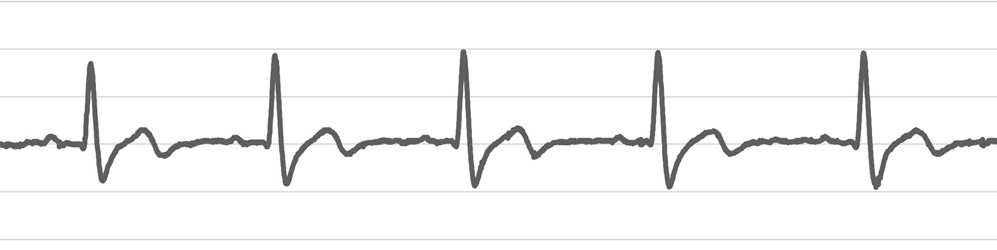
\includegraphics[width=0.7\textwidth]{image1.jpg}
    \caption{心电图示例}
    \label{F.ECG_image}
\end{figure}

然而,传统的心电图检测技术仍面临一些局限,尤其是在便捷性、准确性和实时性方面。传统的心电图检测设备通常需要患者到医院进行检查,这种方式不仅会占用患者大量的时间,还容易造成患者的心电数据在长时间内的缺失或延迟获取。

许多心血管问题,尤其是心律失常等,往往是间歇性或不规律发生的。传统的心电图检测一般是点对点的,即患者在特定的时间和地点进行一次性检测,这样无法捕捉到心脏在不同时间段的动态变化。对于一些潜在的心脏问题,医生往往无法通过单次检查做出全面准确的判断。

如在心血管研究中 \cite{高强度负荷训练对新入伍战士动态心电图相关指标的影响} ,对大量样本的实时同步心电采集的需求逐渐突出,由于传统设备只能同时采集个数样本,所采样本数据难以兼顾时基一致性问题。通过发展无线心电同步采集技术,能够通过无线网络将多台设备同步连接,实时采集患者的心电数据,解决了传统设备空间和连接限制的问题。尤其在大规模监测、远程医疗、运动医学以及急救等领域,无线多心电同步采集设备具有广阔的应用前景 \cite{物联网技术在智能医疗监护与康复辅助设备中的应用探索}。

在国外,随着无线通信技术和心电监测设备的不断进步,无线多心电同步采集系统已经成为心电监护领域的重要研究方向。早期的心电监测设备大多依赖于有线连接,存在安装和使用不便等缺点。而现代无线心电监测设备通过WiFi \cite{基于Wi-Fi的医疗设备物联网采集装置设计} 、蓝牙 \cite{KhoBesar-34} 、Zigbee \cite{I.H.-35} 等无线协议,实现了设备之间的无线互联和远程监控。

国内无线心电同步采集设备的研究起步较晚,早期多为基于有线通信协议的多导联心电同步采集设备 \cite{基于USB的12导联同步心电采集系统} \cite{12导联心电信号同步采集系统} 。近年来随着物联网技术和无线通信协议的进步,国内学者也积极进行相关的理论研究和技术创新,在无线同步采集、信号处理、网络优化等方面取得了一定进展。近年来,随着5G通信技术的推广,心电数据传输的实时性和可靠性有了进一步的提升,尤其是在远程医疗和智能诊断系统的应用中展现出巨大的潜力 \cite{基于“5G+AI”技术的远程心电监测系统研究} 。

尽管国内外都取得了一些进展,但多心电同步采集设备的稳定性、低功耗和高精度等问题依然是当前研究的重点。如何在保证信号采集准确性的同时,提高设备的同步性和抗干扰能力,仍然是一个亟待解决的技术难题。特别是大量设备同时运行的高并发工况,国内外的学术研究却未有过多涉猎,大多只是对此有所提及 \cite{可穿戴心电监测设备的性能评估} \cite{高性能心电信号测量及应用系统的研制} ,而缺乏大量可行性实验数据的支撑。

本项目正是针对多设备心电信号采集中出现的时间同步问题以及多设备并发测量场景为研究重点,进一步推动无线心电同步采集技术的发展

\subsection{主要研究工作}

本研究围绕无线多设备心电信号同步采集系统的关键技术展开,主要包括以下方面:

\begin{enumerate}
    \item \textbf{心电信号采集与硬件优化}
    
    心电图(Electrocardiogram, ECG)信号通过电极接触人体皮肤表面,检测心脏电活动所产生的电位变化。正常的心电波形包含 P 波、QRS 波群和 T 波等,分别对应心脏的不同生理过程。如图 \ref{F.ECG_image2} 所示。

    \begin{figure}[hbt]
        \centering
        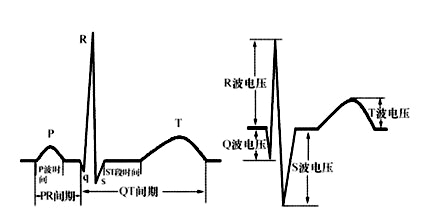
\includegraphics[width=0.6\textwidth]{image2.jpg}
        \caption{心电图各波形、波段示意图}
        \label{F.ECG_image2}
    \end{figure}
    
    本研究针对 ECG 信号采集过程中信号幅值微弱、噪声干扰严重的问题,设计并优化了前端硬件采集电路,包括心电信号的放大、滤波与抗干扰措施。此外,为抑制电磁干扰(Electromagnetic Interference, EMI)并提高系统的电磁兼容性(Electromagnetic Compatibility, EMC),优化了电源管理模块,选型了特定的 DC-DC 转换芯片,降低芯片内部 MOS 管开关频率带来的电源噪声。同时在 PCB layout方面,采用模拟和数字电路分区布线,并通过磁珠单点接地,优化铜铺设和过孔设计,确保模拟信号完整性,减少数字电路和无线射频电路对 ECG 采集电路的干扰。

    \item \textbf{无线通信协议选型}
    
    本研究针对多设备 ECG 数据同步采集的需求,评估了 Wi-Fi、蓝牙及 Zigbee 等主流无线通信协议,并结合其衍生协议(如 Wi-Fi Mesh、Bluetooth Mesh)进行选型优化。为选型合适的无线通信协议,需综合考虑设备最大连接数、通信速率、抗干扰能力以及无线环境部署难度等因素。本研究在初期开发时验证了多种无线通信协议对系统数据同步的影响,并在协议选型基础上优化网络架构,提高数据传输效率,减少数据包延迟,确保系统可在多设备场景下稳定运行。此外,针对设备的配网、连接及断线重连等环节,设计了可靠的设备管理机制,以提高系统的适应性和稳定性。

    \item \textbf{射频性能优化}  
    
    为确保无线射频通信的稳定性与可靠性,本研究对系统的射频特性进行了优化。在PCB设计中连接天线的射频接口使用了IPEX-1接口,方便更换天线进行测试,同时测量并分析了所购买天线的 S 参数、驻波比(Voltage Standing Wave Ratio, VSWR)及回波损耗(Return Loss),确保天线匹配符合通信需求。其次,利用矢量网络分析仪(Vector Network Analyzer, VNA)测量并优化射频匹配网络,通过绘制史密斯圆图(Smith Chart)调整π形匹配网络参数(如串并联适当的电容、电感),查看匹配网络调整后的斯密斯圆图,使系统的特征阻抗接近 50 ohm,降低射频信号的传输反射,提高射频链路的传输效果。

    \item \textbf{多设备数据同步}  
    
    为保证多设备采集数据能够实时重放,无线多设备 ECG 采集系统的开发要点之一是多设备数据的时序同步。由于无线传输具有随机时延,设备间同步误差可能影响 ECG 数据的准确性。本研究针对该问题,设计了基于时间戳同步和统一时钟同步的策略,各节点通过主机构建无线采集网络,并由主机授时,建立统一时基,确保各设备异步采集的各数据所打上的时间戳上具有一致性。

    \item \textbf{低功耗优化}  
    
    本研究充分利用乐鑫公司(Espressif)生产的 ESP32-C3 的低功耗特性,采用 Auto Light-Sleep 模式设计系统休眠与唤醒策略。当操作系统(OS)进入 IDLE 任务且超过设定时间阈值后,系统自动进入 Light-Sleep 模式,以降低功耗。此外,该模式遵循 DTIM(Delivery Traffic Indication Message)机制,使设备能够在保持 Wi-Fi 连接的同时自动唤醒,以确保数据通信的连续性。在此基础上,研究进一步实现了无线发射功率的动态调节,并对系统整体功耗进行评估与优化,从而有效延长设备的续航时间。

    \item \textbf{上位机系统设计}  
    
    上位机程序作为本系统的核心控制平台,承担设备管理、数据监控、实时数据展示及数据存储等关键功能。其主要作用在于实现对多台采集设备的统一调度,并提供直观的数据可视化界面,以满足实时心电信号监测与存储的需求。
    在数据传输方面,上位机程序通过建立 \textit{socket} 连接,实时接收各节点设备发送的UDP数据流,并将心电信号以波形形式展示于用户界面,便于研究人员实时监测受试者的心电状态。此外,用户可在上位机程序中灵活配置采集设备的数量,系统支持多设备的并行管理,能够根据实际需求动态调整系统的工作状态,以适应不同应用场景。
    为进一步提高数据利用价值,上位机程序具备数据存储与导出功能。系统可对采集数据进行存档,并按需导出为 \textit{CSV} 文件格式,每条记录以 [时间戳, 电平数据] 形式存储并按节点序号位列排开,以便后续数据分析与医学诊断。
    
\end{enumerate}
本研究通过上述技术优化,实现了高效、低功耗、稳定的无线 ECG 多设备同步采集系统。

\subsection{论文组织结构}

全文内容共七章,具体内容组织如下:

第一章为绪论。介绍本文的研究背景以及研究意义,对无线心电同步采集技术的国内外研究现状进行梳理与阐述,最后对本文的研究内容与文章结构进行简要概述。

第二章为心电采集的基础理论部分。介绍心电信号的产生原理以及心电信号中P、Q、R、S、T等波形在心电图中的特点,对心电信号的采集、处理等技术进行详细介绍。

第三章为系统总体设计与工作原理,主要介绍了无线多设备心电同步采集系统的总体设计思路、系统架构、硬件设计与实现、软件设计与实现等方面的技术要点。

第四章为采集系统在硬件部分的设计与实现。主要介绍了心电采集的前端硬件设计思路及原理图设计、心电数据处理和发送的主控部分器件选型思路以及原理图设计、天线选型及射频性能调优过程、整板功耗测量实验数据以及功耗优化策略等硬件相关的技术要点。

第五章为采集系统在嵌入式软件部分的设计与实现。主要介绍了系统的软件架构设计、各节点与主机的时序同步策略、节点所采集的心电数据序列化发送策略、低功耗优化策略等软件相关的技术要点。

第六章为采集系统在上位机软件部分的设计与实现。主要介绍了上位机程序的功能设计、数据接收与解析、数据存储与导出、用户界面设计等上位机软件相关的技术要点。

第七章总结与展望,总结了本文的主要工作,展望了下一阶段的研究方向。

\newpage    % 两个章节之间分页,不想分的话可注释掉

\section{相关背景理论知识}

\subsection{心电信号产生原理}

心电信号(Electrocardiographic Signal, ECG)是一种反映心脏电活动的生物电信号,其产生源于心肌细胞膜内外离子的流动,主要涉及钠钠离子(Na$^+$)、钾离子(K$^+$)和钙离子(Ca$^{2+}$)的跨膜转运。心脏的正常电活动由心脏传导系统控制,确保心脏各腔室按照一定的顺序进行兴奋和收缩,从而完成泵血功能。

在正常生理状态下,心脏电活动由窦房结(Sinoatrial Node, SA Node)自动发放的兴奋信号起始,并沿特定的传导路径依次传播至心房和心室,完成整个心动周期。具体而言,窦房结所产生的兴奋首先传导至右心房,引发右心房的去极化与收缩;同时,兴奋通过房间束(Bachmann’s Bundle)传至左心房,导致左心房同步收缩。随后,兴奋沿结间束(Internodal Pathways)传至房室结(Atrioventricular Node)。房室结对兴奋信号产生生理性延迟,以确保心房在心室收缩前充分收缩并完成血液充盈。

兴奋通过房室束(Bundle of His)进入心室传导系统,并沿左、右束支(Left and Right Bundle Branches)迅速传递至浦肯野纤维(Purkinje Fibers),最终激活心室肌,导致心室的去极化和收缩。由于心房与心室之间具有特殊的传导路径,这种传导机制确保兴奋能够在短时间内同步传播至心室各部分,从而实现高效的心脏泵血功能。心脏传导模式如图 \ref{F.ECG_image3} 所示 \cite{现代医学电子仪器原理与设计} 。

\begin{figure}[hbt]
    \centering
    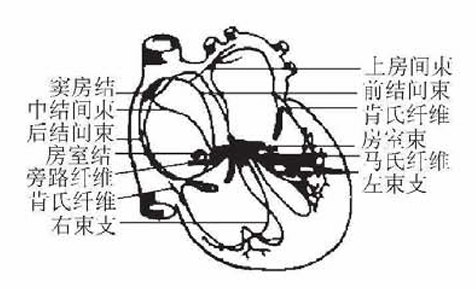
\includegraphics[width=0.6\textwidth]{image3.png}
    \caption{心脏传导系统示意图}
    \label{F.ECG_image3}
\end{figure}

在每一个心动周期中,心脏各部位依照一定的顺序和时间规律经历兴奋的产生、传播和恢复,其电活动表现出方向性、时间性及空间上的特定规律。这些生物电信号可通过心脏周围的导电组织和体液传导至体表,使人体不同部位在每个心动周期中均发生相应的电位变化。心电图(Electrocardiogram, ECG)即是在人体表面特定位置放置电极,以记录这些电信号变化的曲线。心电图能够全面反映心脏兴奋的产生、传导及复极化过程,为心脏功能的评估和疾病诊断提供重要依据。

\subsection{心电图波形特征}

\begin{figure}[hbt]
    \centering
    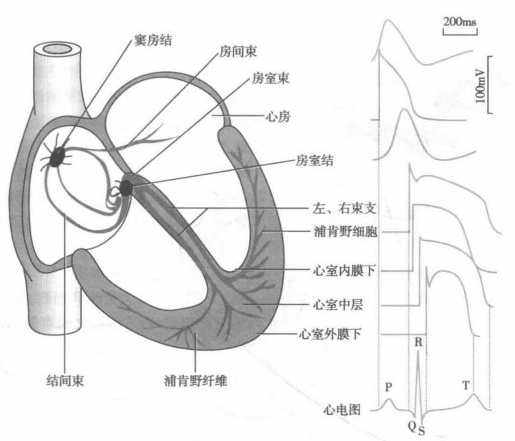
\includegraphics[width=0.6\textwidth]{image4.png}
    \caption{心电图形成示意图}
    \label{F.ECG_image4}
\end{figure}

如图 \ref{F.ECG_image4} 所示 \cite{人体解剖生理学} 心电图(Electrocardiogram, ECG)波形的变化反映了心脏不同阶段的电生理活动。典型的心电图波形包括 P 波、QRS 复合波、T 波和 U 波,如图\ref{F.ECG_image5}所示 \cite{现代医学电子仪器原理与设计} ,各波形的生理意义和正常范围如下:

\begin{enumerate}
    \item \textbf{P波}:P 波由心房去极化产生,其前半部分主要由右心房去极化形成,后半部分主要由左心房去极化形成。正常情况下,P 波的持续时间不超过 0.10 s。

    \item \textbf{P-R间期}:P-R 间期是指 P 波起点到 QRS 复合波起点之间的时间间隔,代表从心房开始兴奋到心室兴奋的时间,即兴奋通过心房、房室结和房室束的传导时间。P-R 间期会随着年龄增长而呈现轻微延长的趋势。

    \item \textbf{QRS复合波}:QRS 复合波反映了左、右心室的去极化过程。QRS 波群的持续时间称为 QRS 时限,代表整个心室肌去极化过程所需的时间。正常情况下,QRS 时限不超过 0.10 s。
    
    \item \textbf{S-T段}:S-T 段是指 QRS 复合波终点到 T 波起点之间的时间区间,代表心室肌复极化的缓慢阶段。正常情况下,该段接近基线,其与基线的偏离一般不超过 0.05 mm。

    \item \textbf{T波}:T 波代表心室肌的复极化过程。在 R 波占主导的心电图中,T 波的幅值应不低于 R 波幅值的 1/10。

    \item \textbf{U波}:U 波出现在 T 波之后,相对基线来说是凹陷的波形,与心室肌复极化后的电位变化相关。
\end{enumerate}

\begin{figure}[hbt]
    \centering
    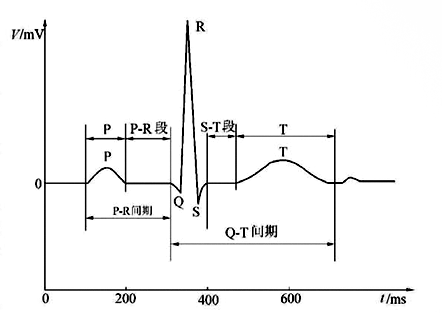
\includegraphics[width=0.6\textwidth]{image5.png}
    \caption{心电图各波段示意图}
    \label{F.ECG_image5}
\end{figure}

\subsection{心电信号采集原理}
在人体体表进行心电图(ECG)记录时,需要解决两个核心问题:一是如何确定电极的放置位置,以确保获得稳定且具有临床价值的信号;二是如何设计电极与放大器的连接方式,以保证信号的准确传输和放大。

\subsubsection{心电图导联方式}

为了实现心电图波形的标准化,提高数据的可比性和诊断的可靠性,临床实践中对电极的放置部位及其连接方式进行了严格规范。按照心电图学的专业术语,电极在人体体表的具体放置方式以及其与放大器的连接形式统称为心电图导联。

心电图导联主要分为标准导联和非标准导联两大类。标准导联是指按照国际标准规定的电极放置位置和连接方式进行心电图记录,包括 I、II、III、aVR、aVL、aVF、V1-V6 等 12 个导联。非标准导联则是指除标准导联之外的其他导联方式,如单极胸导联、肢导联等。

标准导联中I、II、III导联由Einthoven发现,是最早的心电图导联,其原理是利用三个电极在人体体表上的不同位置记录心电信号,以反映心脏的不同方向的电活动。这三个导联的电极放置位置如图\ref{F.ECG_image6}所示 \cite{现代医学电子仪器原理与设计} 。其中,I导联的电极放置在左右手腕,II导联的电极放置在右手腕和左脚踝,III导联的电极放置在左手腕和左脚踝。

\begin{figure}[hbt]
    \centering
    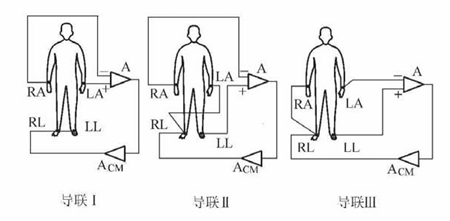
\includegraphics[width=0.6\textwidth]{image6.png}
    \caption{I、II、III导联电极放置示意图}
    \label{F.ECG_image6}
\end{figure}

\subsubsection{心电信号放大与滤波}

心电信号的幅值通常在 0.5 mV 至 5 mV 之间,在采集与传播途中容易夹杂噪声,具有较低的信噪比。为了保证心电信号的准确采集和分析,需要对信号进行适当的放大和滤波处理。最早的心电图机采用机械放大器和滤波器,通过机械装置调节放大倍数和滤波频率,实现对心电信号的处理。随着电子技术的发展,现代心电图机采用电子放大器和滤波器,通过电子元件实现对心电信号的放大和滤波。如图\ref{F.ECG_image7} a,b所示 \cite{现代医学电子仪器原理与设计} ,两种方式的采集前端基本相同,均由电极、放大器和滤波器组成。但是数字滤波器的滤波特性更加灵活,可以根据需要调整滤波频率和滤波类型,实现对心电信号的精确处理,并且可以数字化处理和保存心电信号,方便后续的数据分析和诊断。

\begin{figure}[H]
    \centering
    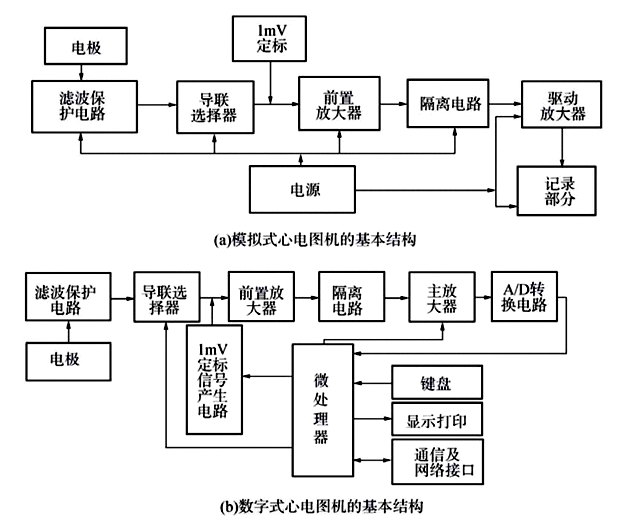
\includegraphics[width=0.8\textwidth]{image7.png}
    \caption{心电信号放大与滤波原理图}
    \label{F.ECG_image7}
\end{figure}

心电信号输入部分包括电极、导联线和前置放大器,其中电极用于接触人体体表,导联线用于传输心电信号。导联线作用是从人体中提取原始的心电信号,并按照导联组合,将信号传输至放大器。导联线将电极片上采集到的心电信号传递到前置放大器,前置放大器对信号进行放大和滤波处理。采取I、II、III导联的话导联线一般是6根,但根据实际使用的话一般只需要使用3根导联线即可完成一种导联的连接。导联线如图\ref{F.ECG_image8}所示,其中红色线为右手腕电极符号为RA或R,黄色线为左手腕电极符号为LA或L,绿色线为左腿电极。

\begin{figure}[hbt]
    \centering
    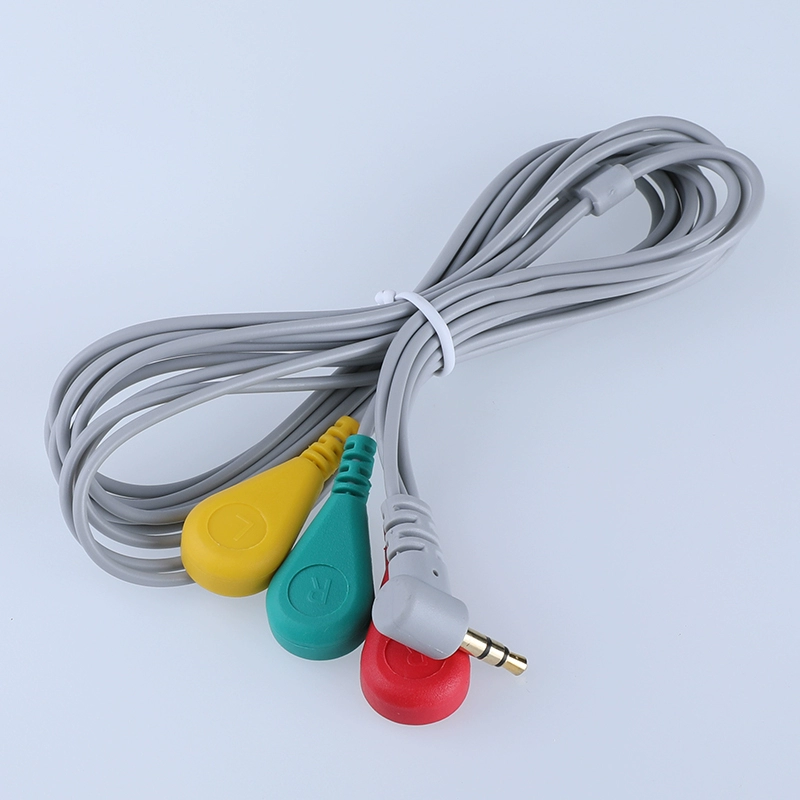
\includegraphics[width=0.4\textwidth]{image8.png}
    \caption{心电采集导联线示意图}
    \label{F.ECG_image8}
\end{figure}

在心电信号的采集与处理过程中,前端放大器起着至关重要的作用。由于人体心电信号的幅度通常处于毫伏(mV)级别,信号较为微弱,且容易受到外界电磁干扰和生理噪声的影响,因此,在信号进入后续处理单元之前,需通过前端放大器进行初步放大,以提高信号的强度和信噪比(SNR),确保后续处理的准确性和稳定性。

前端放大器的主要功能在于将电极采集到的原始心电信号放大至合适的幅度,使其能够满足后续滤波、模数转换(A/D 变换)及数据采集的要求。合理设计的前端放大器不仅应具备高增益特性,还应具有较低的噪声、优良的共模抑制比(CMRR)以及适当的输入阻抗,减少回波反射和信号失真,确保信号的准确采集和传输。心电信号是差模信号,因此前端放大器一般会先通过差分信号放大器突出心电信号的差模成分并移植共模噪声干扰,同时将共模信号通过右腿驱动电路反相放大后输入人体,抵消人体的共模噪声。再通过仪表放大器芯片进行前置放大,提高心电信号的幅值,以便后续的滤波和模数转换。

心电信号中噪声干扰一般是来自于市电工频干扰、人体肌肉电信号干扰、基线漂移等,这些问题会对心电信号的采集和分析造成影响。为了减少这些干扰信号对心电信号的影响,需要对心电信号进行滤波处理。滤波器的作用是通过对心电信号进行滤波,去除掉不需要的频率成分,保留需要的频率成分。心电采集中常用的滤波器有低通滤波器、高通滤波器以及陷波滤波器。低通滤波器的作用主要是去除板级DC-DC电源模块的开关频率带来的电源噪声,高通滤波器的作用主要是去除肌电干扰,肌电干扰是由人体肌肉带动肢体运动产生的不规则高频电干扰,其频率一般在10-1000Hz之间,通过高通滤波器可以去除这部分干扰信号并且可以消除基线漂移。陷波滤波器的作用是滤除特定频率的波形,在心电采集中的作用是去除50Hz市电工频的干扰。

最后通过放大和滤波的心电信号由MCU进行模数转换,将模拟信号转换为数字信号,以便后续的数据处理和存储。

\newpage    % 两个章节之间分页,不想分的话可注释掉


\section{系统总体设计与工作原理}

本系统由心电采集节点设备、基站设备及上位机数据收集监控与控制软件三部分组成,各部分协同工作,以实现高精度、多设备同步的心电信号采集、处理与管理。成功实现了局域网环境下大规模心电采集设备的低延迟、高速率同步采集功能,确保多个心电采集节点间的精确同步,以满足高精度心电数据采集的需求。系统支持 10 台及以上的心电采集设备,并通过基站提供的全局时钟基准,实现不同受试者心电信号的时间同步。各采集节点依据基站发送的时间同步偏移量进行调整,确保所有数据的时间戳一致,从而保证多设备协同工作的高精度同步采集。每个心电采集节点的采样速率可达 1000 Hz,能够高精度记录心电信号的细微变化,同时优化了无线数据传输机制,通过WiFi与上位机建立socket连接,通过UDP发送序列化数据包,保证低延迟数据传输,使系统能够满足实时性要求。与此同时,采集系统配备上位机控制与监测软件,支持灵活配置采集设备数量,满足不同实验环境与应用需求,并具备实时显示心电波形的功能,为研究人员提供直观的监测界面,同时支持数据存储与导出,便于后续信号分析。如图\ref{F.ECG_image9}所示,为系统的功能设计框图。

通过ESP-TOUCH的配网技术以及面向无连接的ESP-NOW通信技术,采集系统能够在不同的网络环境下自动组网,快速部署,并基于无线通信技术降低布线复杂度,提升部署的灵活性和适应性,使其在实验室、医疗机构及远程监测等场景中均能高效、准确地完成心电信号采集。

\begin{figure}[hbt]
    \centering
    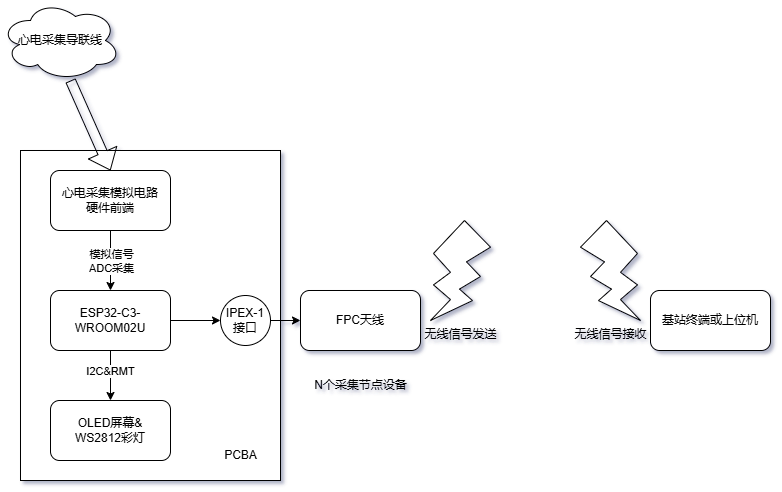
\includegraphics[width=0.8\textwidth]{image9.png}
    \caption{系统功能设计框图}
    \label{F.ECG_image9}
\end{figure}

\subsection{实现心电采集与发送的节点设备}

本设备主要承担心电信号的获取、初步数据处理及数据传输功能,确保心电信号的高质量采集与可靠传输。设备采用单导联心电信号采集方式,通过电极片获取人体生物电信号,并将信号引入板载 3.5mm 耳机接口,经由心电信号采集模拟前端电路进行信号调理,以满足后续数据处理的需求。

在信号处理方面,心电信号首先经过模拟放大电路以提升信号幅度,随后通过低通滤波和带阻滤波电路进行噪声抑制。其中,低通滤波用于去除高频干扰,避免外部电磁干扰对心电波形的影响,而带阻滤波主要针对 50Hz 工频噪声进行抑制,以降低电网干扰对信号的影响。在完成模拟信号的预处理后,信号通过主控芯片ESP32C3的高精度模数转换器(ADC),进行数字化处理。设备支持最高 1000 Hz 采样率,能够精准捕获心电信号的动态变化,满足高分辨率数据分析的需求。

此外,主控芯片内置的 ADC 功能可对采集的心电数据进行基础的数字滤波,以进一步减少环境噪声影响,尤其是开关电源噪声,提高数据的信噪比(SNR)。为确保多设备协同工作的时间一致性,系统在数据传输前对采集数据进行时间戳标记,并以基站提供的全局时钟作为时间基准,使不同采集设备的数据能够保持统一的时间参考,从而确保多设备同步采集的精度和一致性。最后将所采集到的心电数据序列化为数据包,通过 WiFi 与基站建立 socket 连接,以 UDP 协议发送数据包至上位机,实现数据的实时传输。

\subsection{实现时钟同步与组网的基站设备}

基站设备在系统中承担全局时钟同步与设备管理的核心功能,确保所有心电采集节点的时间同步性及网络稳定性。其主要任务是提供全局时钟信号,使系统内的各个采集节点能够按照统一的时间基准进行数据采集,从而确保不同设备之间的心电数据具有严格的时间对齐。在时间同步方面,基站设备利用 ESP-NOW 无线通信协议,在各节点设备逐步加入网络时,向每个新连接的节点提供相应的时间同步偏移量。节点设备接收该偏移量后,依据基站的全局时钟调整自身的本地时间戳,以保证所有节点的数据时间参考一致。这一同步机制有效降低了多设备数据融合时的时间误差,提高了跨设备的心电信号分析精度。

除了时间同步功能,基站设备还负责对整个网络中的设备进行管理和状态监控。基站能够实时显示当前已连接的心电采集设备数量,记录各设备的网络状态,并提供上位机主机的IP 地址、WiFi 连接情况等关键信息,以便于系统运行监测和维护。此外,基站设备还具备网络故障检测能力,可及时发现并报告异常设备,确保系统的稳定性和可靠性。

\subsection{实现数据接收与监控的上位机软件}

上位机程序作为本系统的核心控制平台,主要承担设备管理、数据监控、实时数据展示及数据存储等关键功能,确保系统的灵活配置、数据可视化及长期存储能力。该程序通过网络通信实现对各心电采集设备的实时管理,并为研究人员提供直观的心电信号监测界面,以支持多设备心电数据的同步分析与管理。

在数据通信方面,上位机程序通过Socket建立实时数据接收通道,以UDP方式接收各心电采集节点发送的序列化心电数据包,并基于心电信号的时间戳信息进行数据反序列化,并将数据按时间与电压幅值进行可视化。采集到的数据以心电图波形的形式实时呈现在用户界面上,使研究人员能够直观监测多个受试者的心电信号状态,及时识别异常情况,提高心电数据的临床与科研应用价值。

上位机程序支持多设备并行管理与灵活配置,用户可根据实际需求调整采集设备的数量,实现对不同实验条件或应用场景的适配。系统允许动态添加或移除采集设备,并提供设备状态监控功能,以确保所有节点均处于正常工作状态。 
此外,上位机程序具备数据存储与导出功能,可对采集的心电数据进行本地存储,并支持按需导出CSV文件,数据格式为 [时间戳, 放大后心电信号幅值],以便后续的信号分析与医学诊断。该功能确保心电数据的长期可用性,使研究人员能够在不同时间点对数据进行回溯与深入分析,提高系统的可扩展性和科研应用价值。

\subsection{系统灵活性与易用性设计}

为了满足不同应用场景的需求,本项目特别强调系统的灵活性和易用性,确保设备在多变的应用环境下能够快速部署,并便捷地进行配置和调整。系统的整体设计兼顾了可扩展性、自动化管理以及高效的数据同步,确保多设备协同工作时的稳定性和可靠性。以下是系统在灵活性方面的主要设计特点。

在实际应用中,心电采集设备可能分布于不同地点,且所需的设备数量随应用需求变化而不固定。因此,本系统支持动态调整采集设备的数量,用户可以根据需求自由增减设备,而无需对系统架构进行大幅修改,也无需重新编译或烧录固件,从而提高了系统的适应性和可扩展性。为简化设备的网络配置,系统支持ESP-TOUCH智能配网方案,用户可通过 ESP-TOUCH 手机应用快速完成基站的 Wi-Fi 配置。只需在手机 APP 中输入 Wi-Fi 的名称和密码,基站便可自动连接至指定网络,实现一键式配网,极大地降低了设备部署的复杂性。如图\ref{F.ECG_image10}所示,为ESP-TOUCH示意图。

\begin{figure}[hbt]
    \centering
    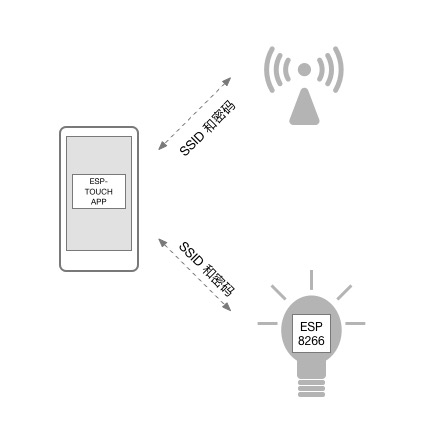
\includegraphics[width=0.6\textwidth]{image10.jpg}
    \caption{ESPTOUCH配网示意图}
    \label{F.ECG_image10}
\end{figure}

系统采用自动组网机制,节点设备与基站设备通过局域网进行无线连接。为提升系统的可扩展性,节点设备无需固定编号,而是由基站根据设备上电顺序进行动态编号分配,从而避免了传统手动编号管理的繁琐操作,并确保设备的接入顺序对系统运行无影响。每个节点设备在启动时,会自动向基站发送连接请求,并在接入网络后根据基站提供的全局时钟信号调整自身的时间基准,以保证所有设备的数据采集同步。即使系统中设备数量发生变化,或部分设备掉线,基站仍可维持全局时间同步,使得新加入或重新连接的节点能够无缝接入,继续采集心电数据,而无需重启整个系统或重新组网。这一机制显著提高了系统的稳定性和容错能力。本系统的设计确保即使各个节点设备在不同时间上电,数据采集仍能保持精准同步。所有采集数据的时间戳均基于基站提供的全局时钟进行标记,确保不同设备间的数据在时间维度上的严格对齐,实现跨设备数据同步。

由于节点设备的启动顺序不受限制,用户可随时启用或关闭任意节点,而无需预先进行设备排序或额外的手动同步操作。基站在检测到新节点接入时,会自动完成时间同步和编号分配,确保该节点能够在当前系统时钟下继续记录数据,而不会影响其他设备的正常采集过程。这一特性不仅增强了系统的灵活性,也使得系统能够适应多变的实验环境和复杂的应用需求,包括远程心电监测、大规模数据采集及实时生理信号分析等场景。

本系统的灵活性设计涵盖了动态设备管理、自动组网、实时时间同步及智能编号分配等方面,使得系统能够在不同网络环境、设备规模及操作流程下高效运行。通过ESP-TOUCH 快速配网、动态节点管理以及基站全局时间同步,系统极大地降低了部署难度,提升了使用便捷性,并确保数据采集的高精度和高可靠性。

\newpage    % 两个章节之间分页,不想分的话可注释掉

\section{硬件部分设计与实现}

\subsection{心电信号采集节点硬件原理图设计}

\subsubsection{主控MCU部分}

主控单元选用乐鑫信息科技(Espressif Systems)推出的ESP32-C3-WROOM-02低功耗无线SoC模组,该芯片集成RISC-V架构32位单核处理器(最高时钟频率160MHz)与2.4GHz无线通信子系统。系统通过其内置的12位高精度SAR型ADC模块(可配置采样率范围4kHz-40kHz)对前端模拟信号处理电路输出的差分心电信号进行数字化转换。模组内建的IEEE 802.11b/g/n Wi-Fi 4协议栈,支持2.4GHz频段的无线通信,可实现与上位机的数据传输。此外,ESP32-C3还集成了丰富的外设接口,包括SPI、I2C、UART、PWM、ADC等,方便与外部传感器、存储器等设备进行通信。

在本系统中节点设备使用了ESP32C3的高精度ADC功能,对心电信号进行模数转换和电池电压采集,并通过芯片内的WiFi基带将心电数据通过2.4GHz频段的无线WiFi网络将心电数据发送至上位机。同时,通过芯片的RMT(Remote Control Transceiver)功能控制板载WS2812的颜色及闪烁频率,实现设备状态的指示。并预留I2C接口,方便后续扩展其他传感器模块,如与血氧测量芯片通信,实现多参数生理信号采集。

为优化开发流程,设计基于沁恒微电子CH343G高速USB-UART桥接芯片的自动下载电路。该电路通过解析上位机通过串口发送的DTR(Data Terminal Ready)和RTS(Request To Send)控制信号,配合RC延时网络(典型值:R=10kΩ,C=100nF)生成符合ESP32-C3启动模式要求的时序组合,并人为切换从Joint Download Boot模式或SPI Boot模式启动,如表\ref{T.ESP32C3-startmode}所示为ESP32C3各启动模式的配置表。此时通过原理图设计,将GPIO2和GPIO8上拉后只需要控制GPIO9的电平即可实现两种启动模式的切换。在ESP32C3的定义中GPIO2、GPIO8、GPIO9都为Strapping Pin,通过控制这三个管脚的电平即可实现不同启动模式的切换。

\begin{table}[htb]
    \centering
    \caption{ESP32-C3启动模式表}
    \label{T.ESP32C3-startmode}
    \begin{tabular}{llll}
    \hline
    启动模式 & GPIO2 & GPIO8 & GPIO9 \\
    \hline
    SPI Boot (default) & 1 & 任意值 & 1 \\
    \hline
    Joint Download Boot & 1 & 1 & 0 \\
    \hline
\end{tabular}
\end{table}

如表\ref{T.ESP32C3-autodownload}所示为ESP32C3自动下载电路的真值表。按照乐鑫官方技术文档\cite{espressif2021esp32c3}可知EN的为电平为0即低电平时芯片关闭,EN为1即高电平时芯片启动。通过控制DTR输出1,RTS输出0,此时GPIO9为1,EN为0,将芯片关闭,延时100ms,再将DTR输出为0,此时EN理应为1,GPIO9为1,芯片启动,不延时立刻将RTS输出为1,此时GPIO9为0,在此刻由于芯片EN脚接入了一个RC延时网络,EN并不会立刻上升为高电平,而是会缓慢上升,当EN的电平上升至0.75的VDD时,芯片启动,此时由于GPIO9的电平为0,芯片进入Joint Download Boot模式。延时50ms将GPIO9这个Strapping Pin维持超过芯片的保持时间$t_H$(如图\ref{F.ECG_image13}所示),等芯片读取完Strapping管脚的电平后再将RTS输出为1,此时EN为1,GPIO9为1,当完成下载并复位芯片时,芯片能够正确从SPI Flash中启动用户代码。通过上述真值表的设计,实现了自动下载电路的功能,方便用户快速烧录固件。

\begin{table}[htb]
    \centering
    \caption{自动下载电路真值表}
    \label{T.ESP32C3-autodownload}
    \begin{tabular}{llllll}
    \hline
    DTR & RTS & EN & GPIO9 \\
    \hline
    0 & 0 & 1 & 1 \\
    \hline
    0 & 1 & 1 & 0 \\
    \hline
    1 & 0 & 0 & 1 \\
    \hline
    1 & 1 & 1 & 1 \\
    \hline
\end{tabular}
\end{table}

\begin{table}[htb]
    \centering
    \caption{Strapping 管脚的时序参数说明}
    \label{T.ESP32C3-strapping}
    \begin{tabular}{|l| p{8cm} |r|} % 3列:左对齐、左对齐、右对齐
    \hline
    \textbf{参数} & \textbf{说明} & \textbf{最小值(ms)} \\
    \hline
    $t_{\mathrm{SU}}$ & 建立时间:拉高 CHIP\_EN 激活芯片前,电源轨达到稳定所需时间 & 0 \\
    \hline
    $t_{\mathrm{H}}$ & 保持时间:CHIP\_EN 已拉高后,strapping 管脚变为
    
    普通 IO 前可读取其值的时间 & 3 \\
    \hline
    \end{tabular}
\end{table}

\begin{figure}[H]
    \centering
    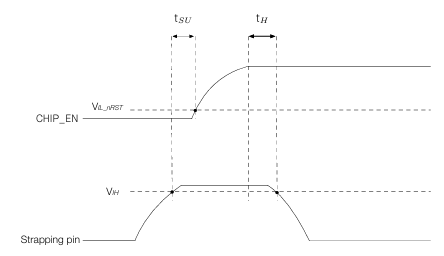
\includegraphics[width=0.6\textwidth]{image13.png}
    \caption{Strapping 管脚时序参数图}
    \label{F.ECG_image13}
\end{figure}

\begin{figure}[hbt]%不知道为什么这个图插入到下一段底下就会报错,只能插入在这里
    \centering
    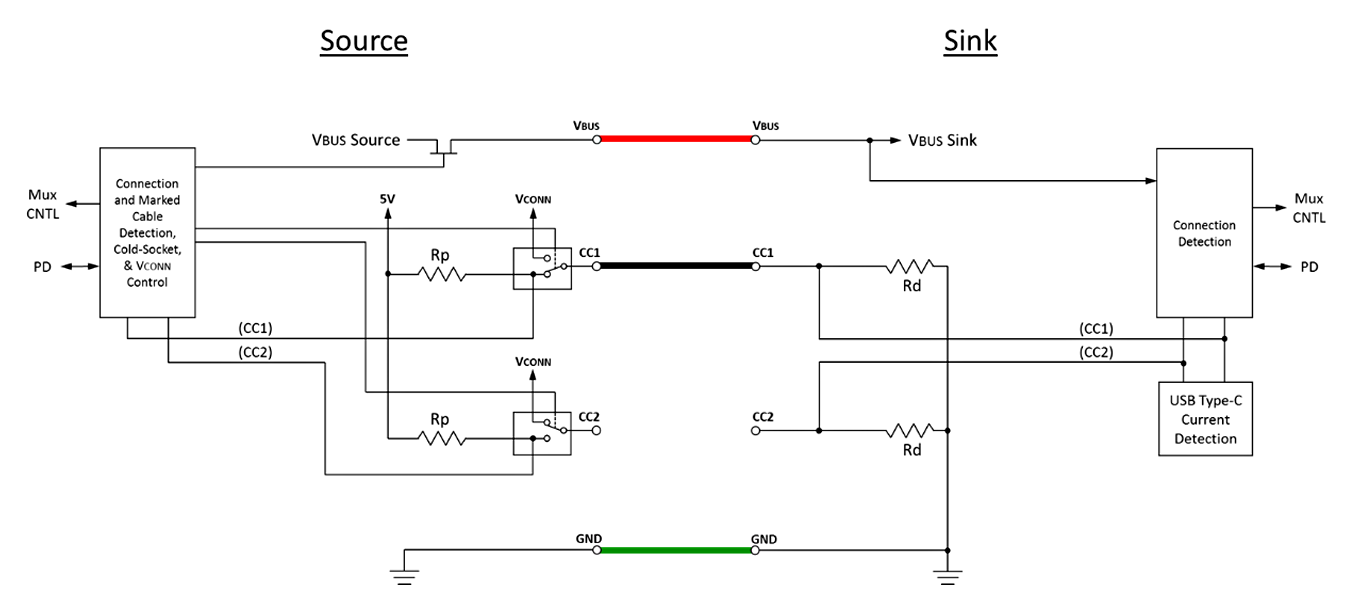
\includegraphics[width=1\textwidth]{image14.png}
    \caption{供电源到Sink设备的功能模式图}
    \label{F.ECG_image14}
\end{figure}

设备采用USB Type-C接口作为标准供电端口,遵循Type-C® Cable and Connector Specification Release 2.4规范。如图\ref{F.ECG_image14} \cite{usbtypec24}所示,在设备端接口CC1、CC2引脚与地之间各配置5.1kΩ±1$\%$精度电阻,形成Rp=5.1kΩ的固定下拉配置,向供电端明确声明本设备作为Sink设备的功率需求等级可向供电设备申请5V/3A的输入到设备中。使得通过C to C线材接入电脑进行调试的同时能够为板载锂电池充电,而避免产生接入后由于Type-C协议不匹配导致无法为设备供电的问题。

本设计通过上述关键技术点的实现,构建了符合医疗电子设备基本要求的硬件平台,其模块化架构便于后续功能扩展与性能优化。如图\ref{F.ECG_image11}所示,为心电信号采集节点硬件原理图设计。

\begin{sidewaysfigure}
    \centering
    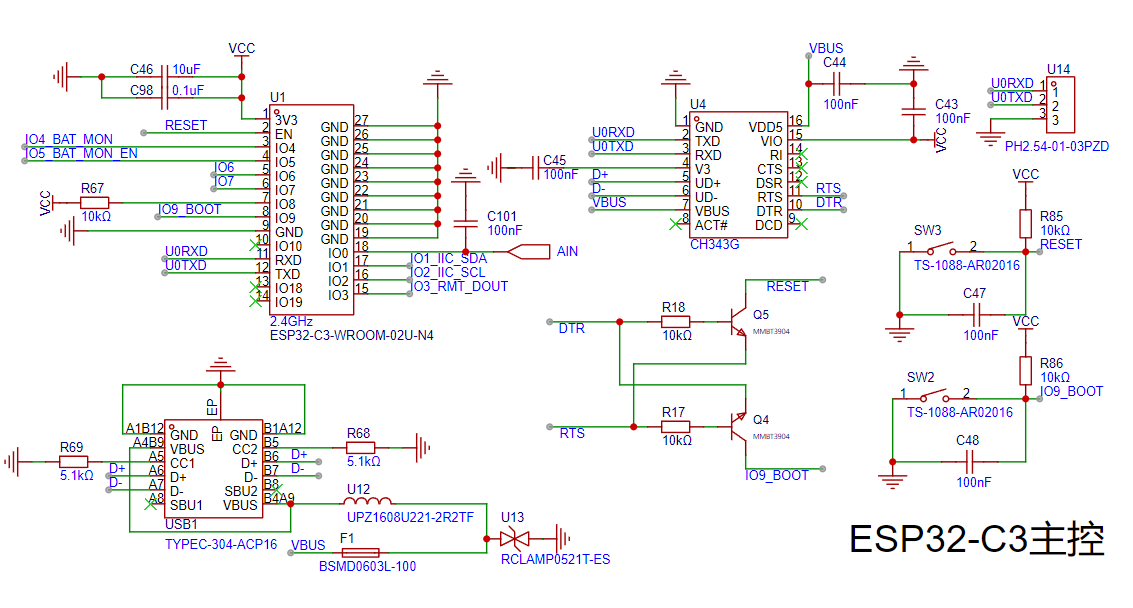
\includegraphics[width=0.8\textwidth]{image11.png}
    \caption{心电信号采集节点硬件原理图设计}
    \label{F.ECG_image11}
\end{sidewaysfigure}



\newpage    % 两个章节之间分页,不想分的话可注释掉

\section{参考文献插入示例}

\LaTeX \cite{lamport1994latex}插入参考文献最方便的方式是使用 \env{bibliography}\cite{pritchard1969statistical}。

大多数出版商的论文页面都会有导出 \format{bib} 格式参考文献的链接,把每个文献的 \format{bib} 放入 \bib{thesis-references.bib},然后用 \oper{bibkey} 即可插入参考文献。

% \lipsum

\newpage    % 两个章节之间分页,不想分的话可注释掉


\section{总结与展望}

\noindent{纯数字编号}
\begin{enumerate}
 \item XXXXXXXXXX
 \label{item1}
 \item XXXXXXXXXX
 \item XXXXXXXXXX
\end{enumerate}
罗马编号
\begin{enumerate}[label=(\roman*)]
 \item XXXXXXXXXX
 \label{item2}
 \item XXXXXXXXXX
 \item XXXXXXXXXX
\end{enumerate}
括号编号
\begin{enumerate}[label=(\arabic*)]
 \item XXXXXXXXXX
 \label{item3}
 \item XXXXXXXXXX
 \item XXXXXXXXXX
\end{enumerate}
半括号编号
\begin{enumerate}[label=\arabic*)]
 \item XXXXXXXXXX
 \label{item4}
 \item XXXXXXXXXX
 \item XXXXXXXXXX
\end{enumerate}
小字母编号
\begin{enumerate}[label=\alph*)]
 \item XXXXXXXXXX
 \label{item5}
 \item XXXXXXXXXX
 \item XXXXXXXXXX
\end{enumerate}

引用测试,正如~\ref{item1}、\ref{item2}、\ref{item3}、\ref{item4}、\ref{item5} 所示

\subsection{工作展望}
手动编号 %(不推荐,无法被交叉引用)

本课题针对XX,鉴于XXX,对XX进行了提高,但是XXX,所以有如下XX:

(1)目前XX虽然XX,但是XX仍然XX,所以XX仍然是一个值得XX的问题。

(2)随着XX,XX具有XX的问题,仍值得进一步XX。

(3)本课题在XX有了XX,但是XX的XX还存在XX,所以XX。


\newpage
